%Este trabalho está licenciado sob a Licença Atribuição-CompartilhaIgual 4.0 Internacional Creative Commons. Para visualizar uma cópia desta licença, visite http://creativecommons.org/licenses/by-sa/4.0/deed.pt_BR ou mande uma carta para Creative Commons, PO Box 1866, Mountain View, CA 94042, USA.

\chapter{Perceptron Multicamadas}\label{cap_mlp}
\thispagestyle{fancy}

\section{Modelo MLP}\label{cap_mlp_sec_modelo}

\hl{Uma Perceptron Multicamadas (MLP, do inglês, \textit{Multilayer Perceptron}) é um tipo de Rede Neural Artificial formada por composições de camadas de perceptrons}. Consulte a Figura \ref{cap_mlp_sec_modelo}.

\begin{figure}[H]
  \centering
  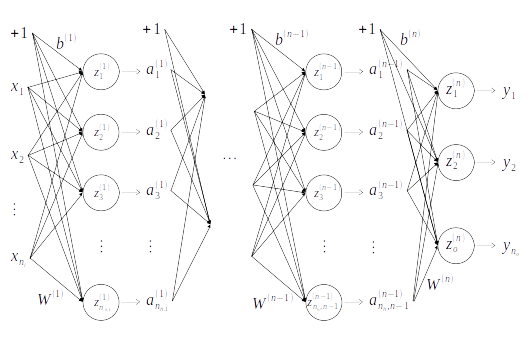
\includegraphics[width=\textwidth]{./cap_mlp/dados/fig_mlp/fig}
  \caption{Estrutura de uma rede do tipo Perceptron Multicamadas (MLP).}
  \label{fig:cap_mlp_sec_modelo:fig:mlp}
\end{figure}

\hl{Denotamos uma MLP de $n$ camadas por}
\begin{align}\hleq
  \pmb{y} = \mathcal{N}\left(\pmb{x}; \left(W^{(l)}, \pmb{b}^{(l)}, f^{(l)}\right)_{l=1}^{n}\right),
\end{align}
onde $\left(W^{(l)}, \pmb{b}^{(l)}, f^{(l)}\right)$ é a tripa de \emph{pesos}, \emph{\textit{biases}} e \emph{função de ativação} da $l$-ésima camada da rede, $l=1, 2, \dotsc, n$.

\hl{A saída da rede é calculada por iteradas composições das camadas}, i.e.
\begin{equation}\hleq
  \pmb{a}^{(l)} = f^{(l)}\underbrace{\left(W^{(l)}\pmb{a}^{(l-1)} + \pmb{b}^{(l-1)}\right)}_{\pmb{z}^{(l)}},
\end{equation}
para $l= 1, 2, \dotsc, n$, denotando $\pmb{a}^{(0)} := \pmb{x}$ e $\pmb{a}^{(n)} := \pmb{y}$.

\subsection{Treinamento}

Fornecido um \emph{conjunto de treinamento} $\{\pmb{x}^{(s)}, \pmb{y}^{(s)}\}_{s=1}^{n_s}$, com $n_s$ amostras, \hl{o treinamento da rede consiste em resolver o problema de minimização}
\begin{equation}\hleq
  \min_{(W,\pmb{b})}\varepsilon\left(\tilde{\pmb{y}}^{(s)}, \pmb{y}^{(s)}\right)
\end{equation}
onde $\varepsilon$ é uma dada \emph{função erro} (em inglês, \textit{loss function}) e $\tilde{\pmb{y}}^{(s)}$, $\pmb{y}^{(s)}$ são as saídas estimada e esperada da $l$-ésima amostra, respectivamente.

\hl{O problema de minimização pode ser resolvido por um }\href{https://notaspedrok.com.br/notas/MatematicaNumericaAvancada/cap\_otimizacao_sec_minimi.html}{\hl{Método de Declive}} e, de forma geral, consiste em:
\begin{enumerate}
\item $W, \pmb{b}$ aproximações iniciais.
\item Para $e\leftarrow 1, \dotsc, n_e$:
  \begin{enumerate}\hleq
  \item $\displaystyle (W, \pmb{b}) \leftarrow (W, \pmb{b}) - l_r\pmb{d}\left(\nabla_{W,\pmb{b}} \varepsilon\right)$
  \end{enumerate}
\end{enumerate}
onde, $n_e$ é o \emph{número de épocas}, $l_r$ é uma dada \emph{taxa de aprendizagem} (em inglês, \textit{learning rate})) e o vetor direção $\pmb{d} = \pmb{d}\left(\nabla_{W,\pmb{b}} \varepsilon\right)$, onde
\begin{equation}\hleq
  \nabla_{W,\pmb{b}} \varepsilon := \left(\frac{\p\varepsilon}{\p W}, \frac{\p\varepsilon}{\p\pmb{b}}\right).
\end{equation}

\hl{O cálculo dos gradientes pode ser feito \emph{de trás para frente}} (em inglês, \textit{backward}), i.e. para os pesos da última camada, temos
\begin{align}
  \hleq{\frac{\p\varepsilon}{\p W^{(n)}}} &\hleq{= \frac{\p\varepsilon}{\p\pmb{y}}\frac{\p\pmb{y}}{\p\pmb{z^{(n)}}}\frac{\p\pmb{z^{(n)}}}{\p W^{(n)}}},\\
                             &= \frac{\p\varepsilon}{\p\pmb{y}}f'\left(W^{(n)}\pmb{a}^{(n-1)}+\pmb{b}^{(n)}\right)\pmb{a}^{(n-1)}.
\end{align}
Para os pesos da penúltima, temos
\begin{align}
  \hleq{\frac{\p\varepsilon}{\p W^{(n-1)}}} &\hleq{= \frac{\p\varepsilon}{\p\pmb{y}}\frac{\p\pmb{y}}{\p\pmb{z^{(n)}}}\frac{\p\pmb{z^{(n)}}}{\p W^{(n-1)}}},\\
                                     &= \frac{\p\varepsilon}{\p\pmb{y}}f'\left(\pmb{z}^{(n)}\right)\frac{\p\pmb{z}^{(n)}}{\p\pmb{a}^{(n-1)}}\frac{\p\pmb{a}^{(n-1)}}{\p\pmb{z}^{(n-1)}}\frac{\p\pmb{z}^{(n-1)}}{\p W^{(n-1)}}\\
                                     &= \frac{\p\varepsilon}{\p\pmb{y}}f'\left(\pmb{z}^{(n)}\right)W^{(n)}f'\left(\pmb{z}^{(n-1)}\right)\pmb{a}^{(n-2)}
\end{align}
e assim, sucessivamente para as demais camadas da rede. \hl{Os gradientes em relação aos \textit{biases} podem ser analogamente calculados}.

\subsection{Aplicação: Problema de Classificação \texttt{XOR}}

Vamos desenvolver uma MLP que faça a operação $\texttt{xor}$ (ou exclusivo). I.e, receba como entrada dois valores lógicos $A_1$ e $A_2$ (V, verdadeiro ou F, falso) e forneça como saída o valor lógico $R = A_1 \texttt{xor} A_2$. Consultamos a seguinte tabela verdade:

\begin{center}
  \begin{tabular}{cc|c}
    $A_1$ & $A_2$ & $R$\\\hline
    V & V & F\\
    V & F & V\\
    F & V & V\\
    F & F & F\\\hline
  \end{tabular}
\end{center}

Assumindo $V = 1$ e $F = -1$, podemos modelar o problema tendo entradas $\pmb{x} = (x_1, x_2)$ e saída $y$ como na seguinte tabela:

\begin{center}
  \begin{tabular}{rr|r}
    $x_1$ & $x_2$ & $y$ \\\hline
    $1$ & $1$ & $-1$ \\
    $1$ & $-1$ & $1$ \\
    $-1$ & $1$ & $1$ \\
    $-1$ & $-1$ & $-1$ \\\hline
  \end{tabular}
\end{center}

\subsubsection{Modelo}

Vamos usar uma MLP de estrutura $2-2-1$ e com funções de ativação $f^{(1)}(\pmb{x}) = \tanh(\pmb{x})$ e $f^{(2)}(\pmb{x}) = id(\pmb{x})$. Ou seja, nossa rede tem duas entradas, uma \emph{camada escondida} com 2 unidades (função de ativação tangente hiperbólica) e uma camada de saída com uma unidade (função de ativação identidade).

\subsubsection{Treinamento}

Para o treinamento, vamos usar a função \hl{\emph{erro quadrático médio}} (em inglês, \textit{mean squared error})
\begin{equation}\hleq
  \varepsilon := \frac{1}{n_s}\sum_{s=1}^{n_s}\left|\tilde{y}^{(s)} - y^{(s)}\right|^2,
\end{equation}
onde os valores estimados $\tilde{y}^{(s)} = \mathcal{N}\left(\pmb{x}^{(s)}\right)$ e $\left\{\pmb{x}^{(s)}, y^{(s)}\right\}_{s=1}^{n_s}$, $n_s=4$, conforme na tabela acima.

\subsubsection{Implementação}

O seguinte código implementa a MLP e usa o \hl{Método do Gradiente Descendente (DG) no algoritmo de treinamento}.

% \lstinputlisting[caption=mlp\_xor.py, label=cap_mlp_sec_modelo:cod:mlp_xor]{./cap_mlp/dados/py_mlp_xor/main.py}
\begin{lstlisting}[caption=mlp\_xor.py, label=cap_mlp_sec_modelo:cod:mlp_xor]
import torch

# modelo

model = torch.nn.Sequential(
    torch.nn.Linear(2,2),
    torch.nn.Tanh(),
    torch.nn.Linear(2,1)
    )

# treinamento

## optimizador
optim = torch.optim.SGD(model.parameters(), lr=1e-2)

## função erro
loss_fun = torch.nn.MSELoss()

## dados de treinamento
X_train = torch.tensor([[1., 1.],
                  [1., -1.],
                  [-1., 1.],
                  [-1., -1.]])
y_train = torch.tensor([-1., 1., 1., -1.]).reshape(-1,1)

print("\nDados de treinamento")
print("X_train =")
print(X_train)
print("y_train = ")
print(y_train)

## num max épocas
nepochs = 5000
tol = 1e-3

for epoch in range(nepochs):

    # forward
    y_est = model(X_train)

    # erro
    loss = loss_fun(y_est, y_train)

    print(f'{epoch}: {loss.item():.4e}')

    # critério de parada
    if (loss.item() < tol):
        break

    # backward
    optim.zero_grad()
    loss.backward()
    optim.step()


# verificação
y = model(X_train)
print(f'y_est = {y}')
\end{lstlisting}

% \subsection{Exercícios}

% [[tag::construcao]]

\section{Aplicação: Aproximação de Funções}\label{cap_mlp_sec_apfun}

\hl{Redes Perceptron Multicamadas (MLP) são aproximadoras universais}. Nesta seção, vamos aplicá-las na aproximação de funções uni- e bidimensionais.

\subsection{Função unidimensional}

Vamos criar uma MLP para aproximar a função gaussiana
\begin{equation}
  y = e^{-x^2},
\end{equation}
para $x\in [-1,1]$.

% \lstinputlisting[caption=mlp\_gaussiana\_1d.py, label=cap_mlp_sec_modelo:cod:mlp_gaussiana_1d]{./cap_mlp/dados/py_mlp_gaussiana_1d/main.py}
\begin{lstlisting}
import torch
import matplotlib.pyplot as plt

# modelo

model = torch.nn.Sequential(
    torch.nn.Linear(1,25),
    torch.nn.Tanh(),
    torch.nn.Linear(25,1)
    )

# treinamento

## fun obj
fobj = lambda x: torch.exp(-x**2)
a = -1.
b = 1.

## optimizador
optim = torch.optim.SGD(model.parameters(),
                        lr=1e-2, momentum=0.9)

## função erro
loss_fun = torch.nn.MSELoss()

## num de amostras por época
ns = 100
## num max épocas
nepochs = 5000
## tolerância
tol = 1e-5

for epoch in range(nepochs):

    # amostras
    X_train = (a - b) * torch.rand((ns,1)) + b
    y_train = fobj(X_train)
    
    # forward
    y_est = model(X_train)

    # erro
    loss = loss_fun(y_est, y_train)

    print(f'{epoch}: {loss.item():.4e}')

    # critério de parada
    if (loss.item() < tol):
        break

    # backward
    optim.zero_grad()
    loss.backward()
    optim.step()


# verificação
fig = plt.figure()
ax = fig.add_subplot()

x = torch.linspace(a, b,
                   steps=50).reshape(-1,1)

y_esp = fobj(x)
ax.plot(x, y_esp, label='fobj')

y_est = model(x)
ax.plot(x, y_est.detach(), label='model')

ax.legend()
ax.grid()
ax.set_xlabel('x')
ax.set_ylabel('y')
plt.show()
\end{lstlisting}

\subsection{Função bidimensional}

Vamos criar uma MLP para aproximar a função gaussiana
\begin{equation}
  y = e^{-(x_1^2 + x_2^2)},
\end{equation}
para $\pmb{x} = (x_1, x_2)\in [-1,1]^2$.

% \lstinputlisting[caption=mlp\_gaussiana\_2d.py, label=cap_mlp_sec_modelo:cod:mlp_gaussiana_2d]{./cap_mlp/dados/py_mlp_gaussiana_2d/main.py}
\begin{lstlisting}
import torch
import matplotlib.pyplot as plt

# modelo

model = torch.nn.Sequential(
    torch.nn.Linear(2,50),
    torch.nn.Tanh(),
    torch.nn.Linear(50,25),
    torch.nn.Tanh(),
    torch.nn.Linear(25,5),
    torch.nn.Tanh(),
    torch.nn.Linear(5,1)
    )

# treinamento

## fun obj
a = -1.
b = 1.
def fobj(x):
    y = torch.exp(-x[:,0]**2 - x[:,1]**2)
    return y.reshape(-1,1)

## optimizador
optim = torch.optim.SGD(model.parameters(),
                        lr=1e-1, momentum=0.9)

## função erro
loss_fun = torch.nn.MSELoss()

## num de amostras por eixo por época
ns = 100
## num max épocas
nepochs = 5000
## tolerância
tol = 1e-5

for epoch in range(nepochs):

    # amostras
    x0 = (a - b) * torch.rand(ns) + b
    x1 = (a - b) * torch.rand(ns) + b
    X0, X1 = torch.meshgrid(x0, x1)
    X_train = torch.cat((X0.reshape(-1,1),
                         X1.reshape(-1,1)),
                        dim=1)
    y_train = fobj(X_train)
    
    # forward
    y_est = model(X_train)

    # erro
    loss = loss_fun(y_est, y_train)

    print(f'{epoch}: {loss.item():.4e}')

    # critério de parada
    if (loss.item() < tol):
        break

    # backward
    optim.zero_grad()
    loss.backward()
    optim.step()


# verificação
fig = plt.figure()
ax = fig.add_subplot()

n = 50
x0 = torch.linspace(a, b, steps=n)
x1 = torch.linspace(a, b, steps=n)
X0, X1 = torch.meshgrid(x0, x1)
X = torch.cat((X0.reshape(-1,1),
               X1.reshape(-1,1)),
              dim=1)

y_esp = fobj(X)
Y = y_esp.reshape((n,n))
levels = torch.linspace(0., 1., 10)
c = ax.contour(X0, X1, Y, levels=levels, colors='white')
ax.clabel(c)

y_est = model(X)
Y = y_est.reshape((n,n))
ax.contourf(X0, X1, Y.detach(), levels=levels)

ax.grid()
ax.set_xlabel('x_1')
ax.set_ylabel('x_2')
plt.show()
\end{lstlisting}

% \subsection{Exercícios}

% [[tag::construcao]]

\section{Aplicação: Equação de Laplace}\label{cap_mlp_sec_eqlaplace}

Vamos criar uma MLP para resolver
\begin{subequations}
  \begin{align}
    -\Delta u &= 0,\quad \pmb{x}\in D = (0, 1)^2,\\
    u &= 0,\quad \pmb{x}\in\p D.
  \end{align}
\end{subequations}

Como exemplo, vamos considerar um problema com solução manufaturada
\begin{equation}
  u(\pmb{x}) = x_1(1-x_1) - x_2(1-x_2).
\end{equation}

\subsection{Diferenças Finitas}

% \lstinputlisting[caption=mlp\_eqlaplace.py, label=cap_mlp_sec_modelo:cod:mlp_eqlaplace]{./cap_mlp/dados/py_mlp_eqlaplace/main.py}
\begin{lstlisting}[caption=mlp\_eqlaplace\_df.py, label=cap_mlp_sec_modelo:cod:mlp_eqlaplace_df]
import torch
import matplotlib.pyplot as plt
import random
import numpy as np

# modelo
model = torch.nn.Sequential(
    torch.nn.Linear(2,50),
    torch.nn.Tanh(),
    torch.nn.Linear(50,10),
    torch.nn.Tanh(),
    torch.nn.Linear(10,5),
    torch.nn.Tanh(),
    torch.nn.Linear(5,1)
)

# SGD - (Stochastic) Gradient Descent
optim = torch.optim.SGD(model.parameters(),
                        lr = 1e-3,
                        momentum = 0.9,
                        dampening = 0.)

# Solução esperada
def u(x, y):
    return a*x*(1-x) - a*y*(1-y)


def laplace_loss(X, U, h2, n, uc=u, p=1.):
    # num de amostras
    nc = 2*n + 2*(n-2)
    ni = n**2 - nc

    # loss interno
    lin = 0.
    for i in range(1,n-1):
      for j in range(1,n-1):
        s = j + i*n
        l = (U[s-n, 0] - 2 * U[s, 0] + U[s+n, 0])/h2 # x
        l += (U[s-1, 0] - 2 * U[s, 0] + U[s+1, 0])/h2 # y
        lin += l**2
    lin /= ni 

    # loss contorno
    lc = 0.
    # 0 <= x <= 1 e y == 0
    for i in range(n):
        s = i*n
        x = M[s,0]
        y = M[s,1]
        lc += (U[s,0] - uc(x,y))**2
    # 0 <= x <= 1 e y == 1
    for i in range(n):
        s = n-1 + i*n
        x = M[s,0]
        y = M[s,1]
        lc += (U[s,0] - uc(x,y))**2
    # 0 == x e 0 < y < 1
    for j in range(1, n-1):
        s = j
        x = M[s,0]
        y = M[s,1]
        lc += (U[s,0] - uc(x,y))**2
    # 1 == x e 0 < y < 1
    for j in range(1, n-1):
        s = j + n*(n-1)
        x = M[s,0]
        y = M[s,1]
        lc += (U[s,0] - uc(x,y))**2
    lc *= p/nc
    
    loss = lin + lc
    return loss

    
# dados do problema

# collocation points
a = 1
n = 11
ns = n**2
h = 1./(n-1)
h2 = h**2

# malha
x = torch.linspace(0, 1, n)
y = torch.linspace(0, 1, n)

M = torch.empty((ns, 2))
s = 0
for i, xx in enumerate(x):
  for j, yy in enumerate(y):
    M[s,0] = xx
    M[s,1] = yy
    s += 1

# gráfico
X, Y = np.meshgrid(x, y)
U_esp = u(X, Y)

# training
nepochs = 10000
nout_loss = 100
nout_plot = 500

for epoch in range(nepochs):

    # forward
    U_est = model(M)

    # loss function
    loss = laplace_loss(M, U_est, h2, n, u, p=10.)

    if ((epoch % nout_loss) == 0):
        print(f'{epoch}: loss = {loss.item():.4e}')
    
    # output current solution
    if ((epoch) % nout_plot == 0):
        # verificação
        fig = plt.figure()
        ax = fig.add_subplot()

        ns = 50
        x1 = torch.linspace(0., 1., ns)
        x2 = torch.linspace(0., 1., ns)
        X1, X2 = torch.meshgrid(x1, x2)
        # exact
        Z_esp = torch.empty_like(X1)
        for i,x in enumerate(x1):
            for j,y in enumerate(x2):
                Z_esp[i,j] = u(x, y)
        c = ax.contour(X1, X2, Z_esp, levels=10, colors='white')
        ax.clabel(c)

        X_plot = torch.cat((X1.reshape(-1,1),
                            X2.reshape(-1,1)), dim=1)
        Z_est = model(X_plot)
        Z_est = Z_est.reshape((ns,ns))
        cf = ax.contourf(X1, X2, Z_est.detach(), levels=10, cmap='coolwarm')
        plt.colorbar(cf)
        
        ax.grid()
        ax.set_xlabel('$x_1$')
        ax.set_ylabel('$x_2$')
        plt.show()        

    # backward
    optim.zero_grad()
    loss.backward()
    optim.step()
\end{lstlisting}

\subsection{Autograd}

\begin{lstlisting}[caption=mlp\_eqlaplace\_ag.py, label=cap_mlp_sec_modelo:cod:mlp_eqlaplace_ag]
import torch
import matplotlib.pyplot as plt
import random
import numpy as np

# modelo
model = torch.nn.Sequential(
    torch.nn.Linear(2,50),
    torch.nn.Tanh(),
    torch.nn.Linear(50,10),
    torch.nn.Tanh(),
    torch.nn.Linear(10,5),
    torch.nn.Tanh(),
    torch.nn.Linear(5,1)
)

# SGD - (Stochastic) Gradient Descent
optim = torch.optim.SGD(model.parameters(),
                        lr = 1e-3,
                        momentum = 0.9,
                        dampening = 0.)

# Solução esperada
def u(x, y):
    return a*x*(1-x) - a*y*(1-y)


def laplace_loss(X, U, h2, n, uc=u, p=1.):
    # num de amostras
    nc = 2*n + 2*(n-2)
    ni = n**2 - nc

    # loss interno
    lin = 0.
    for i in range(1,n-1):
      for j in range(1,n-1):
        s = j + i*n
        x = X[s:s+1,:].detach()
        x.requires_grad = True
        u = model(x)
        grad_u = torch.autograd.grad(u, x,
                                     create_graph = True,
                                     retain_graph = True)[0]
        u_x = grad_u[0,0]
        u_y = grad_u[0,1]

        u_xx = torch.autograd.grad(u_x, x,
                                   create_graph = True,
                                   retain_graph = True)[0][0,0]
        u_yy = torch.autograd.grad(u_y, x,
                                   create_graph = True,
                                   retain_graph = True)[0][0,1]
        lin = torch.add(lin, (u_xx + u_yy)**2)
    lin /= ni 

    # loss contorno
    lc = 0.
    # 0 <= x <= 1 e y == 0
    for i in range(n):
        s = i*n
        x = M[s,0]
        y = M[s,1]
        lc += (U[s,0] - uc(x,y))**2
    # 0 <= x <= 1 e y == 1
    for i in range(n):
        s = n-1 + i*n
        x = M[s,0]
        y = M[s,1]
        lc += (U[s,0] - uc(x,y))**2
    # 0 == x e 0 < y < 1
    for j in range(1, n-1):
        s = j
        x = M[s,0]
        y = M[s,1]
        lc += (U[s,0] - uc(x,y))**2
    # 1 == x e 0 < y < 1
    for j in range(1, n-1):
        s = j + n*(n-1)
        x = M[s,0]
        y = M[s,1]
        lc += (U[s,0] - uc(x,y))**2
    lc *= p/nc
    
    loss = lin + lc
    return loss

    
# dados do problema

# collocation points
a = 1
n = 11
ns = n**2
h = 1./(n-1)
h2 = h**2

# malha
x = torch.linspace(0, 1, n)
y = torch.linspace(0, 1, n)

M = torch.empty((ns, 2))
s = 0
for i, xx in enumerate(x):
  for j, yy in enumerate(y):
    M[s,0] = xx
    M[s,1] = yy
    s += 1

# gráfico
X, Y = np.meshgrid(x, y)
U_esp = u(X, Y)

# training
nepochs = 10000
nout_loss = 100
nout_plot = 500

for epoch in range(nepochs):

    # forward
    U_est = model(M)

    # loss function
    loss = laplace_loss(M, U_est, h2, n, u, p=10.)

    if ((epoch % nout_loss) == 0):
        print(f'{epoch}: loss = {loss.item():.4e}')
    
    # output current solution
    if ((epoch) % nout_plot == 0):
        # verificação
        fig = plt.figure()
        ax = fig.add_subplot()

        ns = 50
        x1 = torch.linspace(0., 1., ns)
        x2 = torch.linspace(0., 1., ns)
        X1, X2 = torch.meshgrid(x1, x2)
        # exact
        Z_esp = torch.empty_like(X1)
        for i,x in enumerate(x1):
            for j,y in enumerate(x2):
                Z_esp[i,j] = u(x, y)
        c = ax.contour(X1, X2, Z_esp, levels=10, colors='white')
        ax.clabel(c)

        X_plot = torch.cat((X1.reshape(-1,1),
                            X2.reshape(-1,1)), dim=1)
        Z_est = model(X_plot)
        Z_est = Z_est.reshape((ns,ns))
        cf = ax.contourf(X1, X2, Z_est.detach(), levels=10, cmap='coolwarm')
        plt.colorbar(cf)
        
        ax.grid()
        ax.set_xlabel('$x_1$')
        ax.set_ylabel('$x_2$')
        plt.show()        

    # backward
    optim.zero_grad()
    loss.backward()
    optim.step()
\end{lstlisting}

% \subsection{Exercícios}

% [[tag::construcao]]
